% !TeX spellcheck = ru_RU
% !TEX root = vkr.tex

\section{Исследование производительности tokio}

Целями следующих экспериментов является выявление возможной зависимости пропускной способности рантайма от взаимодействия воркеров с глобальной очередью.

\subsection{Ход исследования}

Для проверки гипотезы об ограничении производительности ресурсами одного рантайма, были произведены измерения пропускной способности системы, состоящей из нескольких рантаймов приведенной приведенные на графике \ref{fig:tatlin:multi_rt:eval}. Задачи производились потоками воркеров --- добавлялись в глобальную очередь при переполнении пачками. Каждое измерение использовало одинаковое количество системных потоков разделяемое между рантаймами.

\begin{figure}[H]
    \begin{center}
        \makebox[\textwidth]{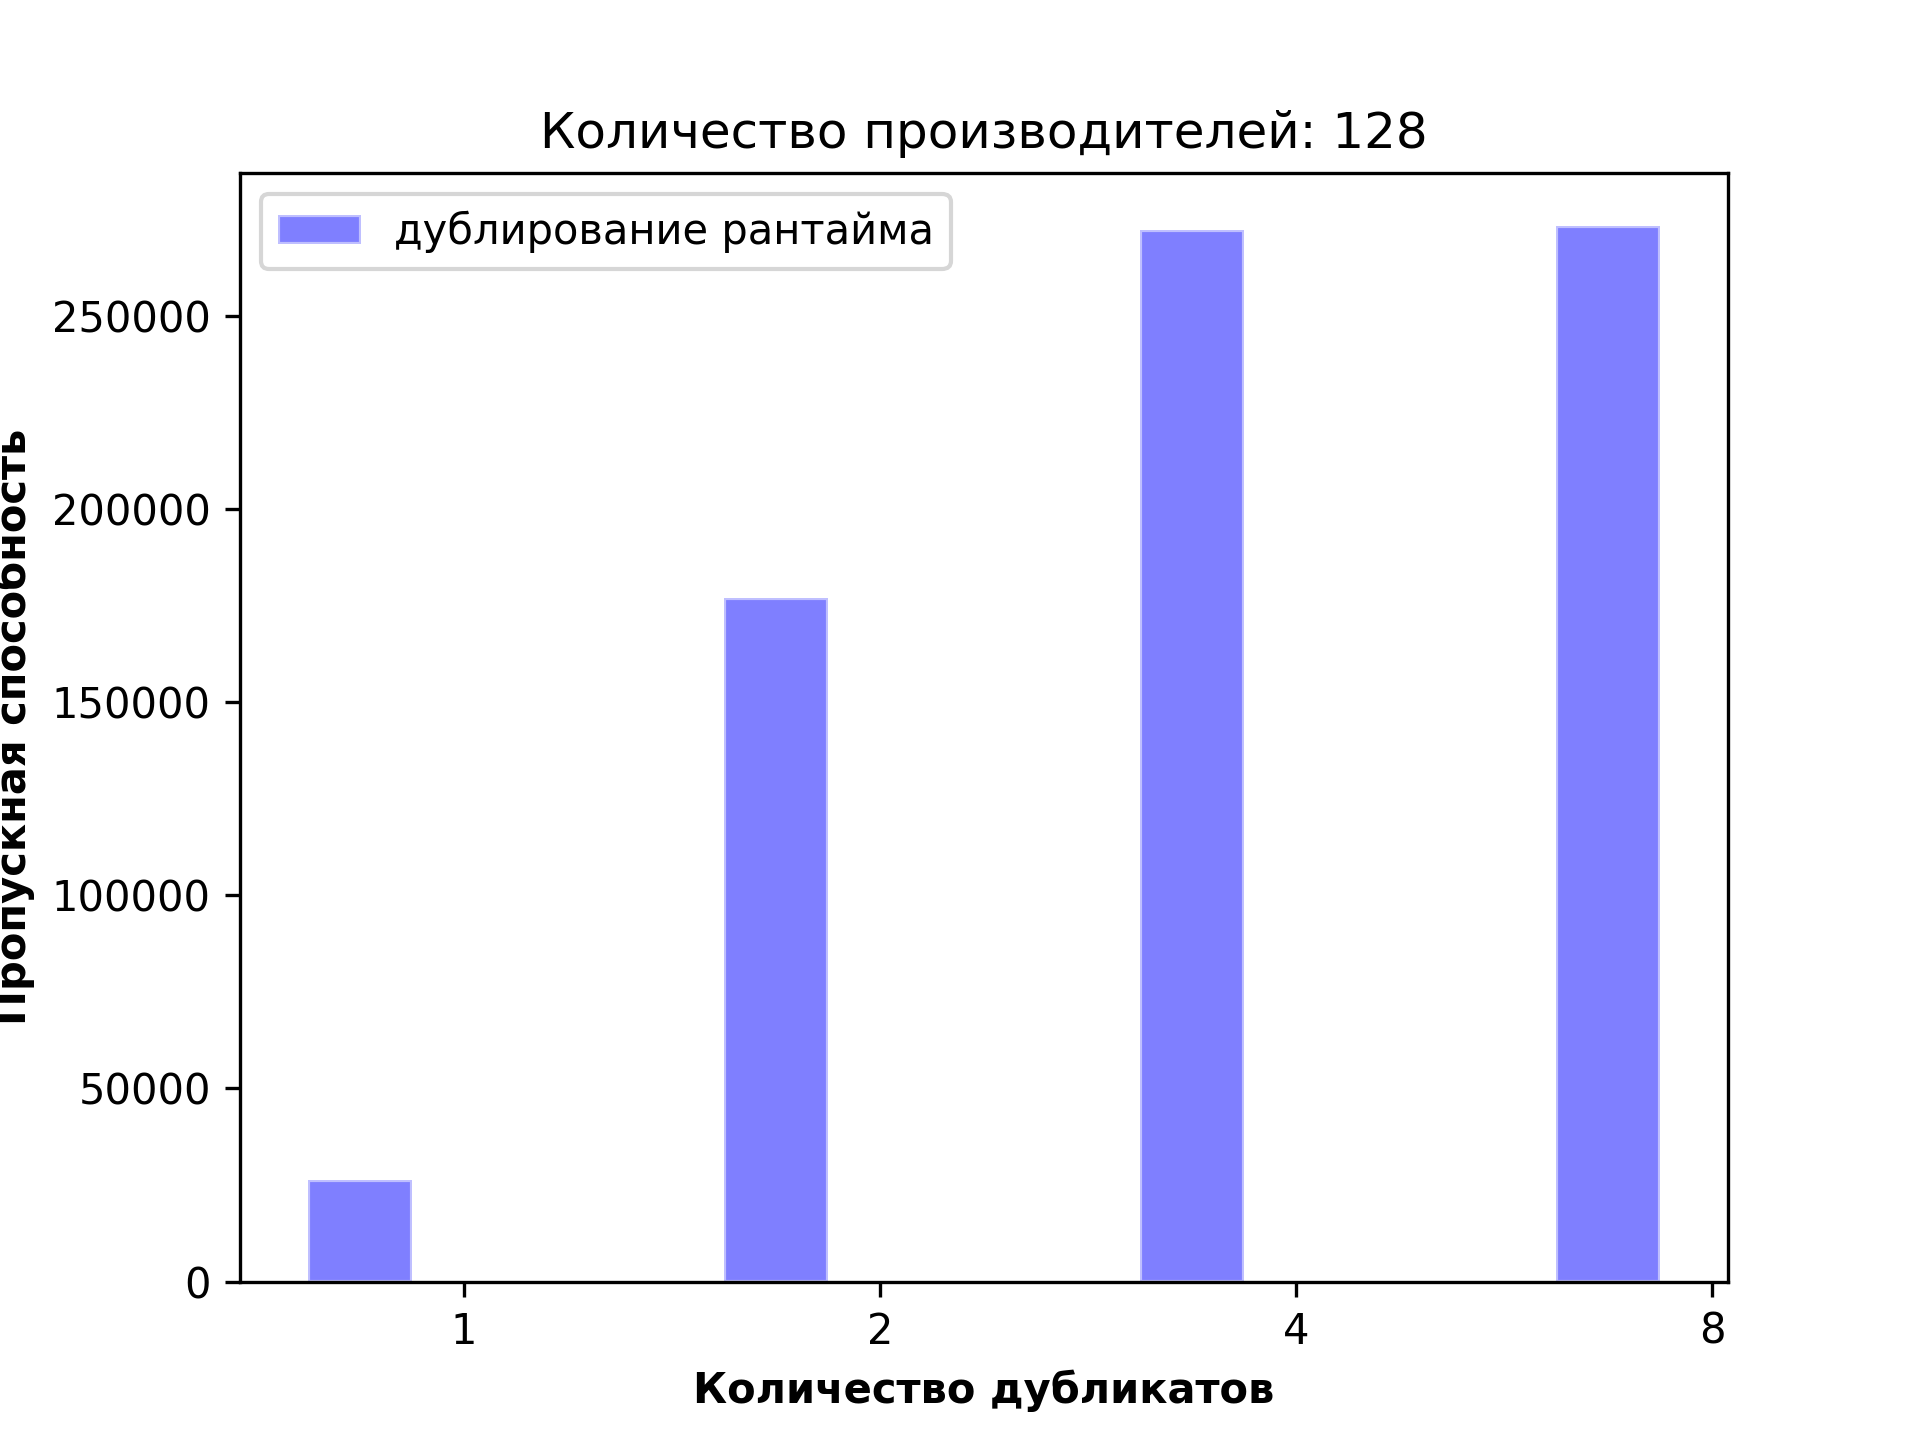
\includegraphics[scale=0.80]{pictures/rt_128_1000.png}}
    \end{center}

    \caption{Производительность системы при использовании нескольких рантаймов}
    \label{fig:tatlin:multi_rt:eval}
\end{figure}

Из изображения заметным становится увеличение производительности пропорционально количеству рантаймов.

\subsection{Вывод}

Глобальная очередь может накладывать ограничение на производительность всего рантайма.

\begin{itemize}
    \item При дубликации ресурсов --- использовании нескольких инстансов tokio рантайма, наблюдается увеличение пропускной способности. Что может быть связано со многими факторами:
    \begin{itemize}
        \item Если глобальная очередь действительно накладывает ограничения на пропускную способность, то с увеличением количества рантаймов меньшее количество воркеров конкурирует за глобальную очередь в каждом инстансе.
        \item Увеличение пропускной способности так же может наблюдаться по другим причинам, например, конкуренция потоков воркеров при регистрация задачи в различных инстансах рантайма рантаймах может быть ниже: задачи все еще получают уникальные индентификаторы в процессе, однако теперь используются разные инстансы \verb|OwnedQueue|.
    \end{itemize}
    \item Существуют ресурсы tokio разделяемые между различными инстансами, например статическая атомарная переменная используемая для генерирации индентификаторов задач.
\end{itemize}
